\chapter{Digital Pāḷi Dictionary (DPD)}\label{chap:dpd}

A remarkable Pāli dictionary nowadays is undoubtedly the DPD.\footnote{\url{digitalpalidictionary.github.io}, \url{dpdict.net}} This dict is so complex that we have to treat it differently. Formerly, the DPD was released only dict data that can be used with dict programs like StarDict or GoldenDict. That makes integration to the program difficult. Finally, it has been released in SQLite DB format as well. This makes the integration much easier.

However, due to the massive size of the DPD data and its activeness in updating, we cannot bundle the data with the program. The inevitable solution is we have to download and process the data before use.

\section{Downloading DPD}

The easiest way to get the DPD data is using the internal DPD downloader/installer invoked by menu DPD > {\faSix \symbol{"F381}} Download DPD database. If you have updated online info as mentioned in Section \ref{sect:updating} and launch the downloader, a window as shown in Figure \ref{fig:dpd-downloader} will pop up.

\begin{figure}[!hbt]
\centering
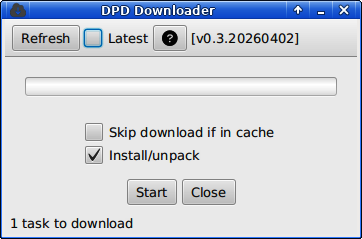
\includegraphics[width=0.6\linewidth]{images/dpd-downloader.png}\\
\caption{DPD Downloader}
\label{fig:dpd-downloader}
\end{figure}

If this downloader has been opened before the online data is updated, before you continue you should press Refresh button to renew the URL data. The download URL provided is supposedly of the newest DPD, as its version shown in the tool bar. But this may not be the most recent because the updating cycle of the DPD is quick and often ahead of the program's update. If you know that there is a more recent version, you can select the \emph{Latest} option. Now then the downloader will get the latest one instead.\footnote{There are some risk of using the latest download because it is not tested properly, but possibility of a crash or incompatibility is low.}

What to do next is just hit the Start button and wait until the installation is finished.

\boxnote{If you just want to download the DPD data into the program's cache without installation, make the option {\faSixReg \symbol{"F0C8}} \emph{Install/unpack} unchecked.\\
\hspace{5mm}If you want to install an existing downloaded file in the cache without downloading a new one, make the option {\faSixReg \symbol{"F14A}} \emph{Skip download if in cache} checked and {\faSixReg \symbol{"F14A}} \emph{Install/unpack} checked.
}

\section{Using DPD}

Just downloading the DPD database is not enough for the program to use the data effectively. Only some data are available, such as Roots, which reads the database directly. To make use of the whole data, you have to process it further for both groups of data: dictionary and deconstructor.

\subsection{Dictionary}

The dictionary entries of DPD are now around 460,000 items available to search (the real head words that have definitions are around 90,000). To use this data efficiently, we have to optimize it by creating a new database with more streamlined tables. This database is called \texttt{PP-DPD}. Before you can do this, you have to open DPD Dictionary window first.

\dothis{To open DPD Dictionary window, press {\ppicons D}\ button in the main tool bar, or use this menu:\\
\menucommand{DPD > {\ppicons D}\ Dictionary}
}

Once you get DPD Dictionary window, the first thing to do is to generate tables by pressing {\faSix \symbol{"F7D9}} Generate button. The process can take a while. After it is done, now you can enter a word to search. Moreover, after the creation the MDPD in Dictionaries will be also available.

\boxnote{After the {\faSix \symbol{"F7D9}} Generate button is pressed to create DPD related tables, the Mini-DPD (MDPD) will be also available in Dictionaries window.}

Figure \ref{fig:dpd-dictionary} shows an example result from one searching. The search is always incremental, so it needs time for the first letter's results to be retrieved.

\begin{figure}[!hbt]
\centering
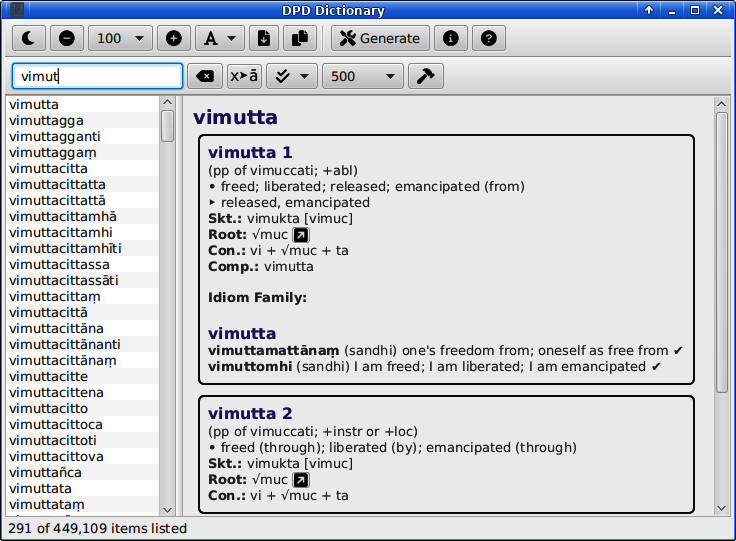
\includegraphics[width=0.9\linewidth]{images/dpd-dictionary.png}\\
\caption{DPD Dictionary window}
\label{fig:dpd-dictionary}
\end{figure}

If you have ever seen a search result of DPD in its web (\url{dpdict.net}) or in dict programs, you will feel unfamiliar but relieved here. Unnecessary information is screened out, and the display is made clean and simple.\footnote{If the users find that some important information is left out and should be added here, feel free to tell the author.} This can make you more focused on what is important, less distracted. For the full information of DPD entries, please use your dict programs or use the web version.

\boxnote{There are two modes of searching: search from term start and search within term. The option can be set by pressing {\faSix \symbol{"F560}} button. There are also some other options here. Please learn by doing.\\
\hspace{5mm}Another option that can affect the search performance is the maximum results (shown as a number, e.g., 500). Using a great number retards the search.\\
\hspace{5mm}The user can add search results from Deconstructor table (see below), if available, by using {\faSix \symbol{"F6E3}} toggle button.
}

\subsection{Deconstructor}

Another interesting feature of DPD is the deconstructor, a dictionary of compounds (\pali{samāsa}) and joined words (\pali{sandhi}). Now the entries of this list are over 860,000 items. To use this dictionary, you have to open the deconstructor window first, by menu DPD > {\faSix \symbol{"F6E3}} Deconstructor.

\dothis{To open DPD Deconstructor window, use this menu:\\
\menucommand{DPD > {\faSix \symbol{"F6E3}} Deconstructor}
}

Like the DPD Dictionary, before you can issue any search, you have to create the deconstructor's optimized table first, by pressing {\faSix \symbol{"F7D9}} Generate button and wait for a while. When deconstructor data is ready, the result is listed immediately in Pāli order (see Figure \ref{fig:dpd-deconstructor}). You can change the maximum number of results by the menu button provided. And you can filter the result by entering some query. Three modes of search filter are available: (1) search by term's start, (2) search by term's within, and (3) search both by term's and deconstruction's within. The last mode can be a little slow.

\begin{figure}[!hbt]
\centering
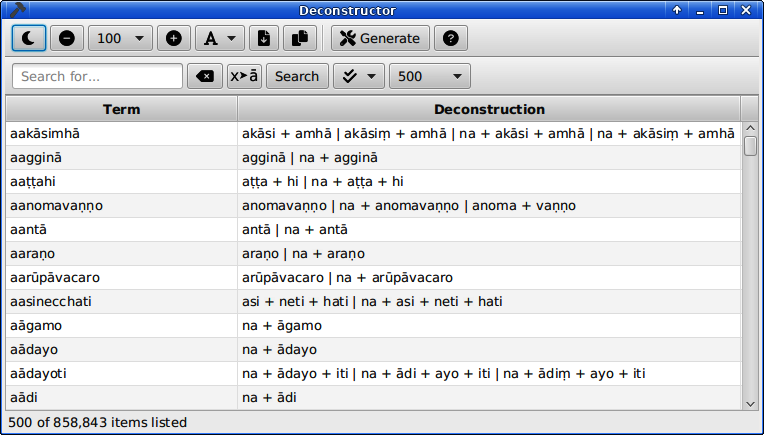
\includegraphics[width=0.9\linewidth]{images/dpd-deconstructor.png}\\
\caption{DPD Deconstructor window}
\label{fig:dpd-deconstructor}
\end{figure}

\newpage
\boxnote{After the optimized data of DPD Dictionary and Deconstructor are created, it is a good practice to lock the PP-DPD database by toggling this menu:\\
\menucommand{DPD > {\faSix \symbol{"F09C}} PP-DPD DB unlocked}\\
to\\
\menucommand{DPD > {\faSix \symbol{"F023}} PP-DPD DB locked}\\
\\
Now then the {\faSix \symbol{"F7D9}} Generate button in both windows will be disabled.
}

\subsection{Other tools}

Apart from the main two groups of data mentioned above, we can access other information by listing them in tables. Available data are all DPD head words, Pāli roots as organized by the DPD, and families of terms.

The DPD head words are those having definitions and detailed information. These data get retrieved when you search in the dictionary. If you just want to see the list, open the head-word window by menu DPD > {\faSix \symbol{"F521}} Head words. The window is shown in Figure \ref{fig:dpd-headwords}.

\begin{figure}[!hbt]
\centering
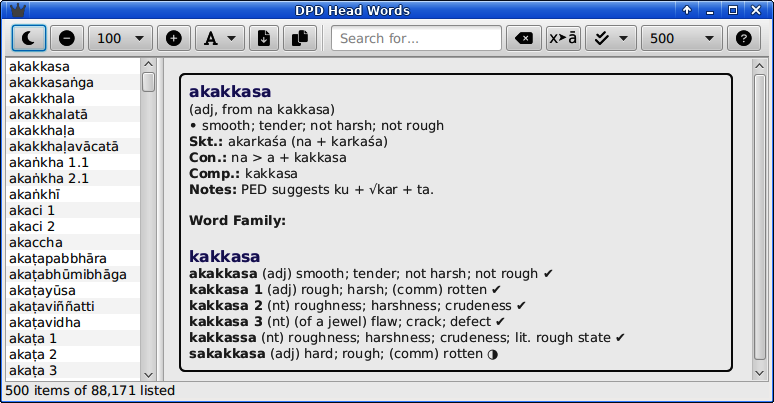
\includegraphics[width=0.9\linewidth]{images/dpd-headwords.png}\\
\caption{DPD Head words}
\label{fig:dpd-headwords}
\end{figure}

In a similar manner, roots that are listed in the DPD can be shown all at once in Roots window (see Figure \ref{fig:dpd-roots}), by menu DPD > {\faSix \symbol{"F4D8}} Roots.

\begin{figure}[!hbt]
\centering
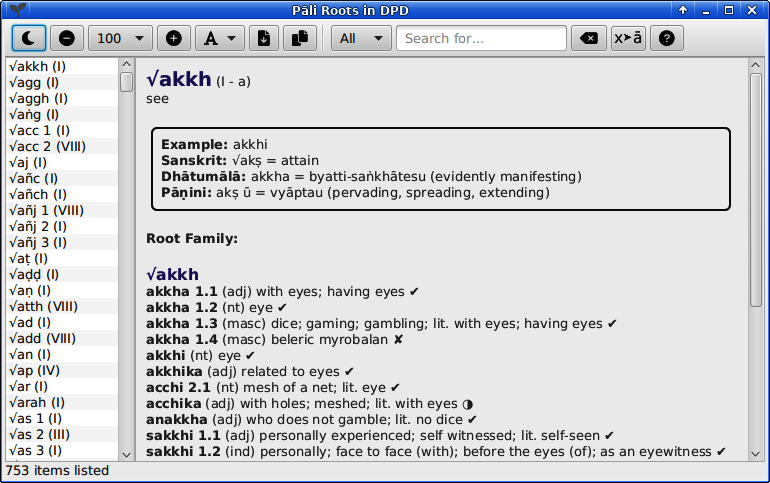
\includegraphics[width=0.9\linewidth]{images/dpd-roots.png}\\
\caption{DPD Roots}
\label{fig:dpd-roots}
\end{figure}

Students of Pāli and Buddhism will enjoy the collections of various data in the DPD, known as \emph{families of terms}. These include compound family, word family, idiom family, and set family. Whereas the word and idiom family can also be shown in the result of DPD Dictionary, other families are listed only in the families window. You can open this window by menu DPD > {\faSix \symbol{"F468}} Families of terms. An example of a family of a word set can be seen in Figure \ref{fig:dpd-families}.

\begin{figure}[!hbt]
\centering
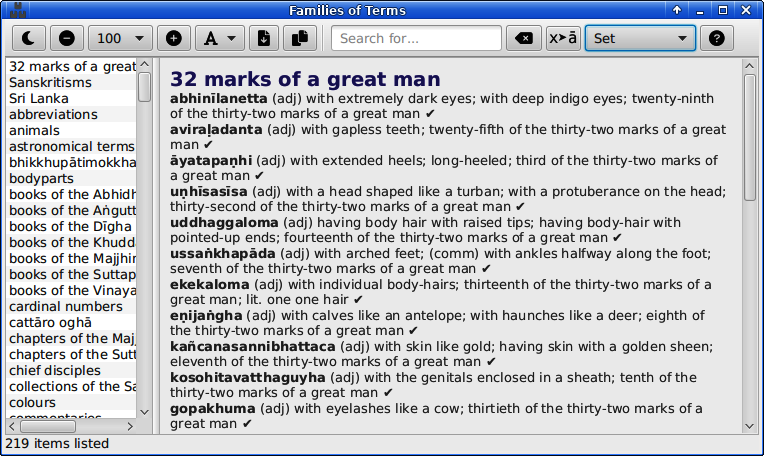
\includegraphics[width=0.9\linewidth]{images/dpd-families.png}\\
\caption{A family of a word set}
\label{fig:dpd-families}
\end{figure}

\section{Manual installation}

It is possible that you can intall the DPD database manually by yourselves without using the provided downloader. Here are what to do:

\newpage
\dothis{To install DPD database manually, follow these steps:\\
\begin{compactenum}
\item Go to the DPD releases.\footnote{\url{github.com/digitalpalidictionary/dpd-db/releases}}
\item Find the most recent (or a preferred) release and download \texttt{dpd-mobile-db.zip} from its assets.\footnote{Formerly, we have used the full \texttt{dpd.db}, but now it seems unavailable. Fortunately, nothing is missing in the mobile database, and it is much smaller in size.}
\item Unpack the \texttt{zip} file with a suitable program, resulting in \texttt{dpd-mobile.db}.
\item Copy the \texttt{dpd-mobile.db} to directory \texttt{data/db} in the program's root.
\item Check the database's applicability.
\end{compactenum}
}

Checking the database's applicability should be done in case you download the version newer than the program's preset. If the result is negative, you should revert the database to an older version. To check the applicability, follow the box below.

\newpage
\dothis{To check the applicability of DPD after downloading and unpacking it, use this menu:\\
\menucommand{DPD > {\faSix \symbol{"F0F1}} Check DB applicability}\\
}

Alternatively, you can check the applicability by using \mbox{DpdUtil} (see Section \ref{sect:dpdutil} on page \pageref{sect:dpdutil}).
